\section{Estado del arte}

\begin{slide}
  \begin{block}{\textbf{Interacción}}
    \begin{itemize}
      \item Explícita
      \item Implícita
    \end{itemize}
  \end{block}
  \begin{block}<2>{\textbf{Paradigmas de interacción}}
    \begin{itemize}
      \item Ordenador de sobremesa
      \item Computación ubicua
      \item Realidad virtual
      \item Realidad aumentada
    \end{itemize}
  \end{block}
\end{slide}

\begin{slide}
  Ordenador de sobremesa
  \begin{figure}[!h]
    \begin{center}
      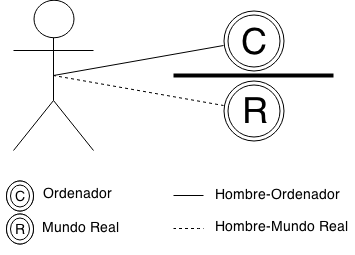
\includegraphics[height=0.6\textheight]{img/IGU.png}
    \end{center}
  \end{figure}
\end{slide}

\begin{slide}
  Computación ubicua
  \begin{figure}[!h]
    \begin{center}
      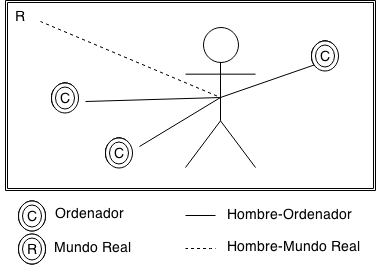
\includegraphics[height=0.6\textheight]{img/CU.png}
    \end{center}
  \end{figure}
\end{slide}

\begin{slide}
  Realidad virtual
  \begin{figure}[!h]
    \begin{center}
      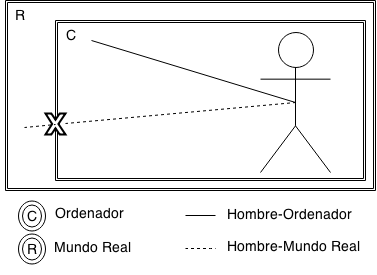
\includegraphics[height=0.6\textheight]{img/RV.png}
    \end{center}
  \end{figure}
\end{slide}

\begin{slide}
  Realidad aumentada
  \begin{figure}[!h]
    \begin{center}
      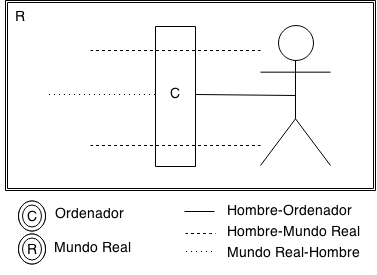
\includegraphics[height=0.6\textheight]{img/RA.png}
    \end{center}
  \end{figure}
\end{slide}

\begin{slide}
  \begin{block}{\textbf{Sistemas de navegación por satélite}}
    \begin{itemize}
      \item NAVigation System and Ranging - Global Position System (NAVSTAR-GPS)
      \item Global’naya Navigatsionnaya Sputnikovaya Sistema (GLONASS)
    \end{itemize}
  \end{block}
\end{slide}

\begin{slide}
  Trilateración
  \begin{figure}[!h]
    \begin{center}
      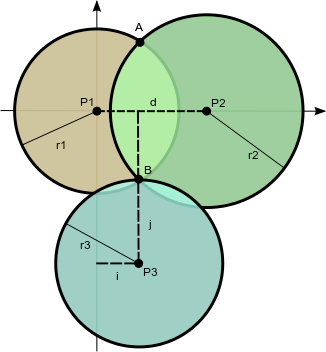
\includegraphics[height=0.7\textheight]{img/trilateracion.png}
    \end{center}
  \end{figure}
\end{slide}

\begin{slide}
  \begin{block}{\textbf{Plataformas smartphone}}
    \begin{center}
      \begin{minipage}[b]{0.4\linewidth}
        \begin{center}
          \begin{figure}[!h]
            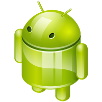
\includegraphics[height=0.25\textheight]{img/android.png}
          \end{figure}
          Android (81\%)
        \end{center}
      \end{minipage}
      \vspace{0.5cm}
      \begin{minipage}[b]{0.4\linewidth}
        \begin{center}
          \begin{figure}[!h]
            
\includegraphics[height=0.25\textheight]{img/ios.png}
          \end{figure}
          iOs (12,9\%)
        \end{center}
      \end{minipage}
      \begin{minipage}[b]{0.4\linewidth}
        \begin{center}
          \begin{figure}[!h]
            
\includegraphics[height=0.25\textheight]{img/wphone.png}
          \end{figure}
          Windows Phone (3,7\%)
        \end{center}
      \end{minipage}
      \begin{minipage}[b]{0.4\linewidth}
        \begin{center}
          \begin{figure}[!h]
            
\includegraphics[height=0.25\textheight]{img/blackberry.png}
          \end{figure}
          Blackberry (1,7\%)
        \end{center}
      \end{minipage}
    \end{center}
  \end{block}
\end{slide}

\begin{slide}
  \begin{block}{\textbf{Wearables}}
    \begin{itemize}
      \item Perfiles bluetooth
      \item Bluetooth con aplicación propietaria
      \item Bluetooth con Google Play Services
    \end{itemize}
  \end{block}
\end{slide}

% Local Variables:
%  TeX-master: "main.tex"
%  coding: utf-8
%  mode: latex
%  mode: flyspell
%  ispell-local-dictionary: "castellano8"
% End:
